% Created 2022-12-09 Fri 16:03
% Intended LaTeX compiler: pdflatex
\documentclass[11pt]{article}
\usepackage[utf8]{inputenc}
\usepackage[T1]{fontenc}
\usepackage{graphicx}
\usepackage{grffile}
\usepackage{longtable}
\usepackage{wrapfig}
\usepackage{rotating}
\usepackage[normalem]{ulem}
\usepackage{amsmath}
\usepackage{textcomp}
\usepackage{amssymb}
\usepackage{capt-of}
\usepackage{hyperref}
\usepackage{minted}
\author{Curtis D'Alves}
\date{Fall 2017}
\title{CAS 750 Model Based Image Reconstruction Final Report}
\hypersetup{
 pdfauthor={Curtis D'Alves},
 pdftitle={CAS 750 Model Based Image Reconstruction Final Report},
 pdfkeywords={},
 pdfsubject={},
 pdfcreator={Emacs 28.2 (Org mode 9.4.6)}, 
 pdflang={English}}
\begin{document}

\maketitle
\newpage
\section{Introduction}
\label{sec:orgb88e20d}
Magnetic resonance imaging (MRI) is a method for image reconstruction that
involves collecting data in a frequency domain (a.k.a k-space) and converting
it into the spatial domain. This is done via the Inverse Fourier Transform, a
mathematical transform that decomposes functions into their frequency
components. Because of mechanical constraints, conventional MRI's deliberately
under-sample data in order to reduce scan times. This under-sampling renders a
simple Inverse Fourier Transform insufficient, requiring an optimization
problem to reconstruct the image over an appropriately devised model.
Techniques for constructing and evaluating such models will be discussed,
including code for solving these problems using an optimization library /
language we developed known as HashedExpression.


\section{Simple De-noising Reconstruction}
\label{sec:org6986886}

Image reconstruction models for MRI need to consider under-sampling in k-space
(i.e., lost signals). Figure \ref{fig:LostSignal} illustrates this lose of signal

\begin{figure}[!htpb]
\centering
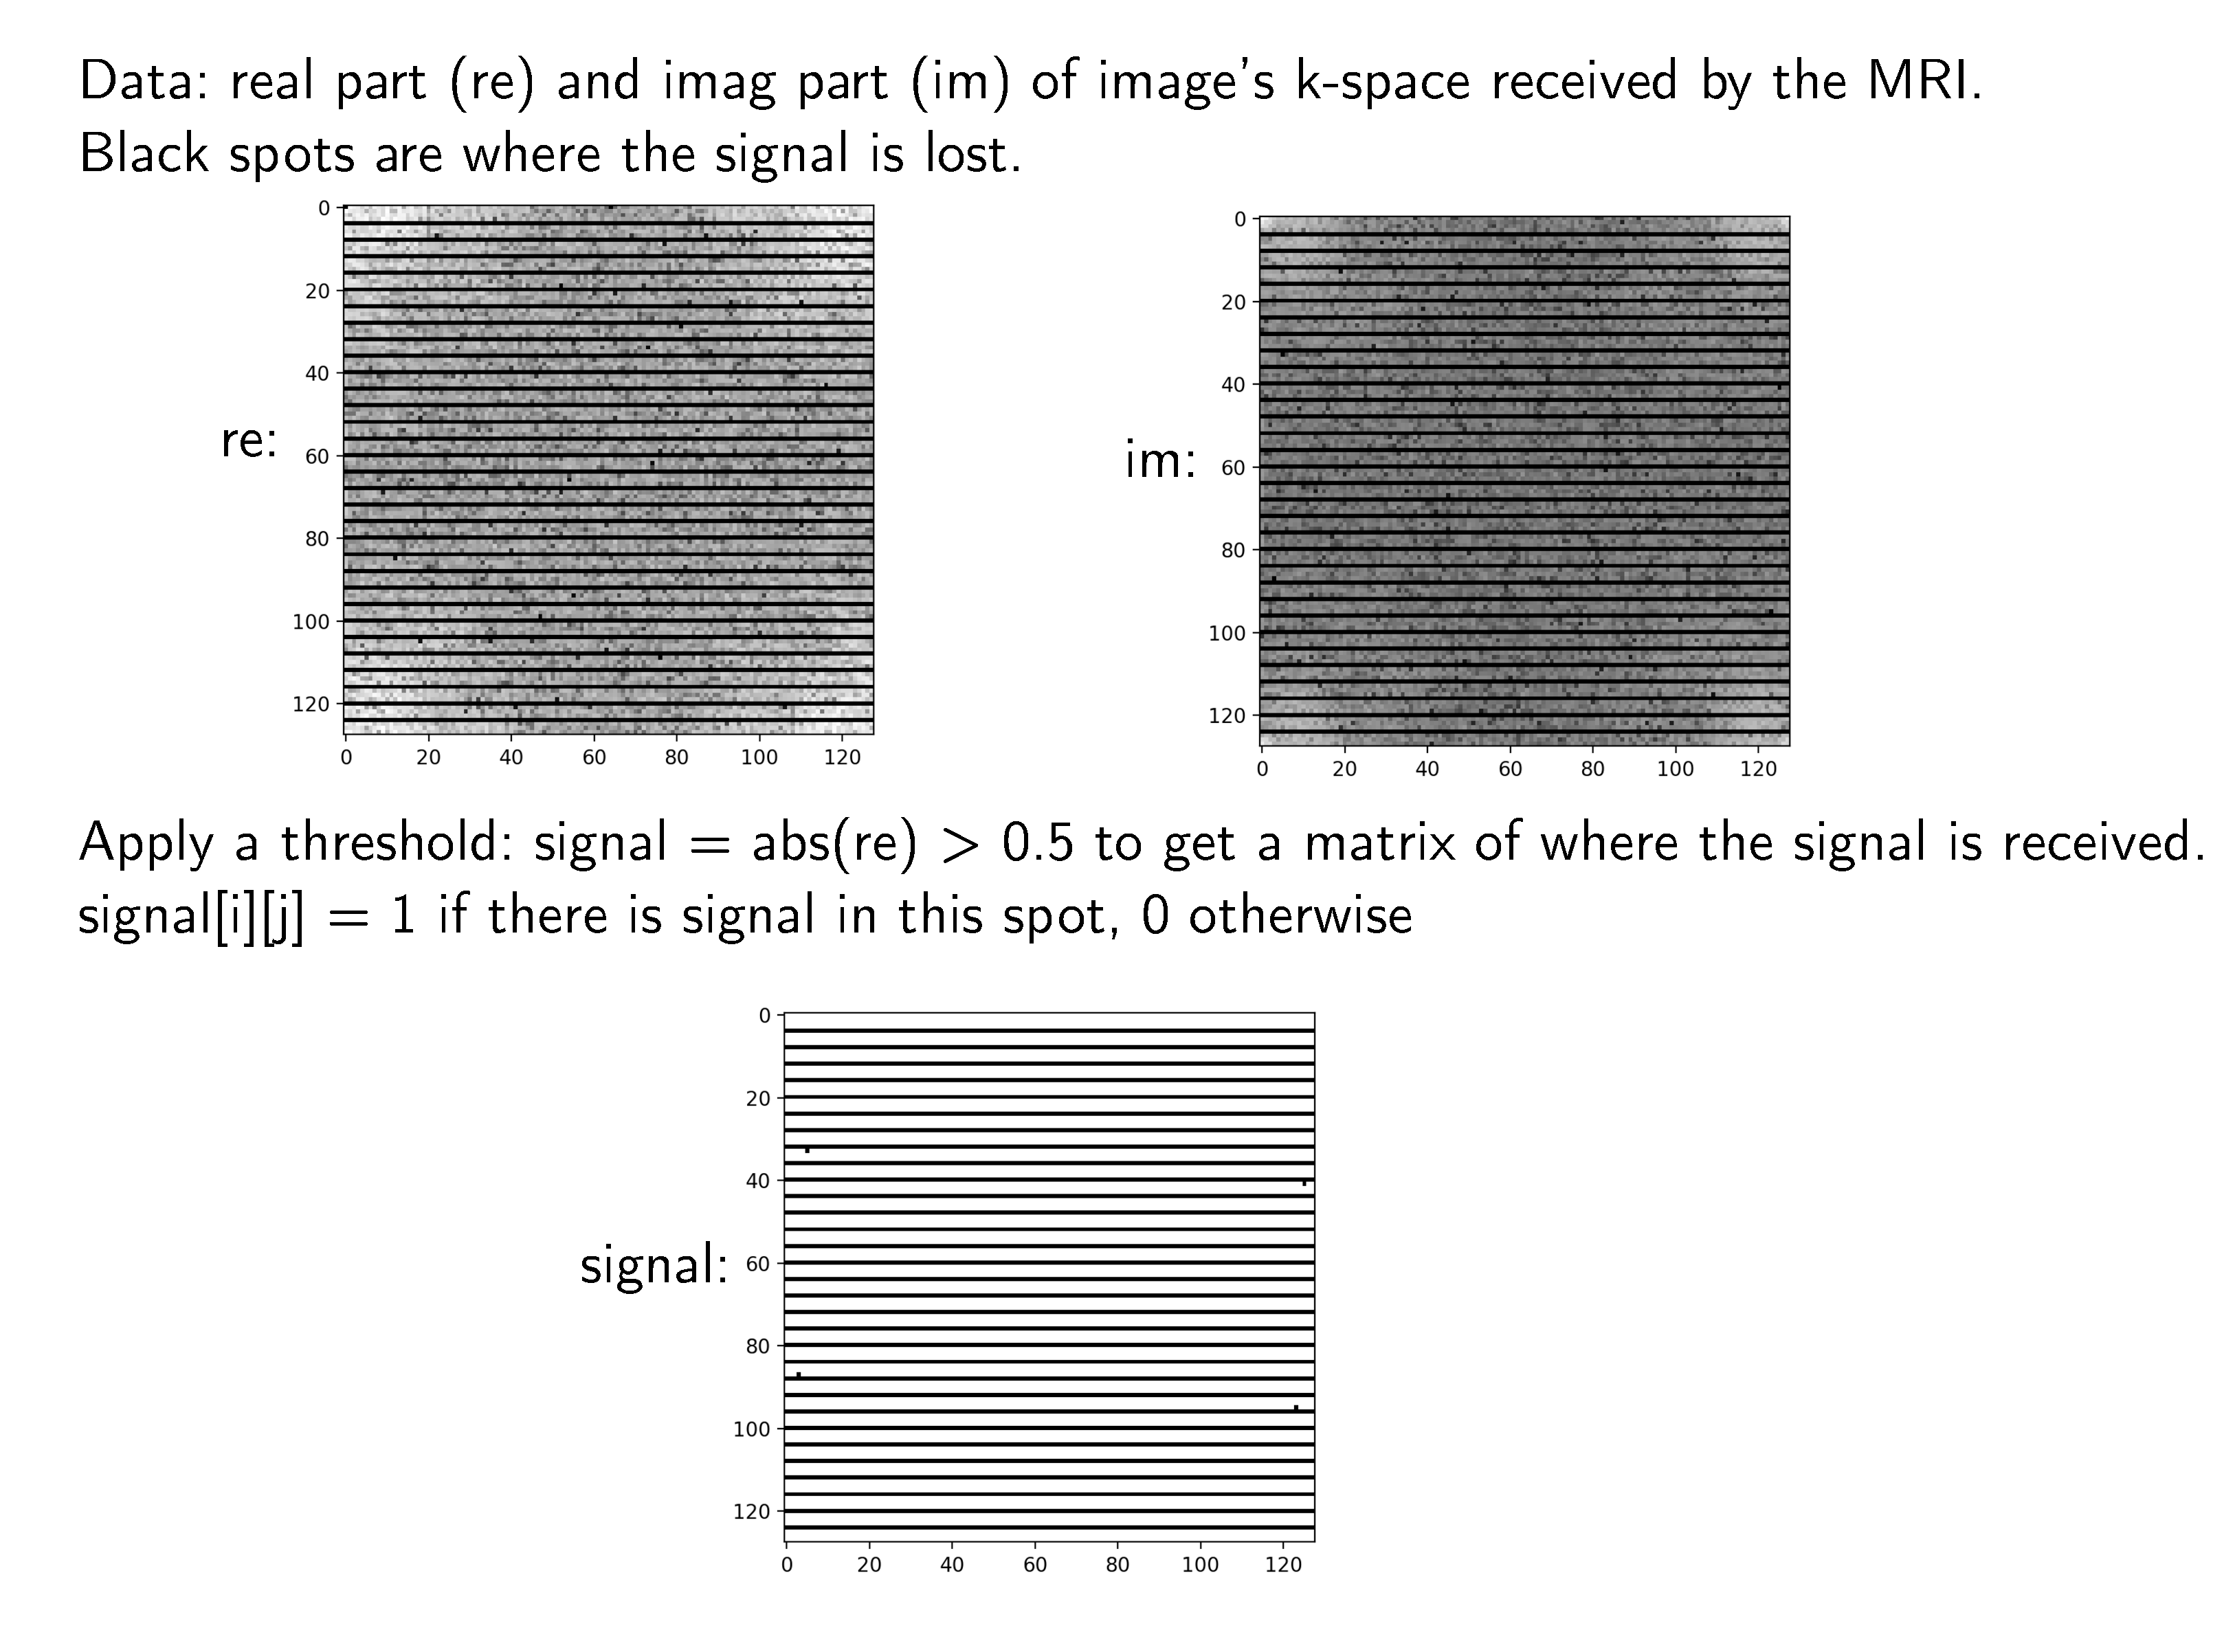
\includegraphics[width=0.5\textwidth]{figs/MRIBrain1.pdf}
\caption{\label{fig:LostSignal}Lost Signal}
\end{figure}

We can perform a naive image reconstruction using an inverse FFT (Fast Fourier
Transform) on the image in question. The resulting image will contain noise,
the goal of a simple optimization model is to de-noise the resulting image. An
example model over some given data \(y\) and resulting image \(x\) is

\begin{equation}
| FT(x) - y | ^2 + \lambda(f(y)) |
\end{equation}

where \(f(y)\) is some regularizer (such as the l2-norm) and \(\lambda\) is a scaling.

To demonstrate this technique, we have taken a picture of brain that we
artificially add noise to, see \ref{fig:BrainBefore}

\begin{figure}[!htpb]
\centering
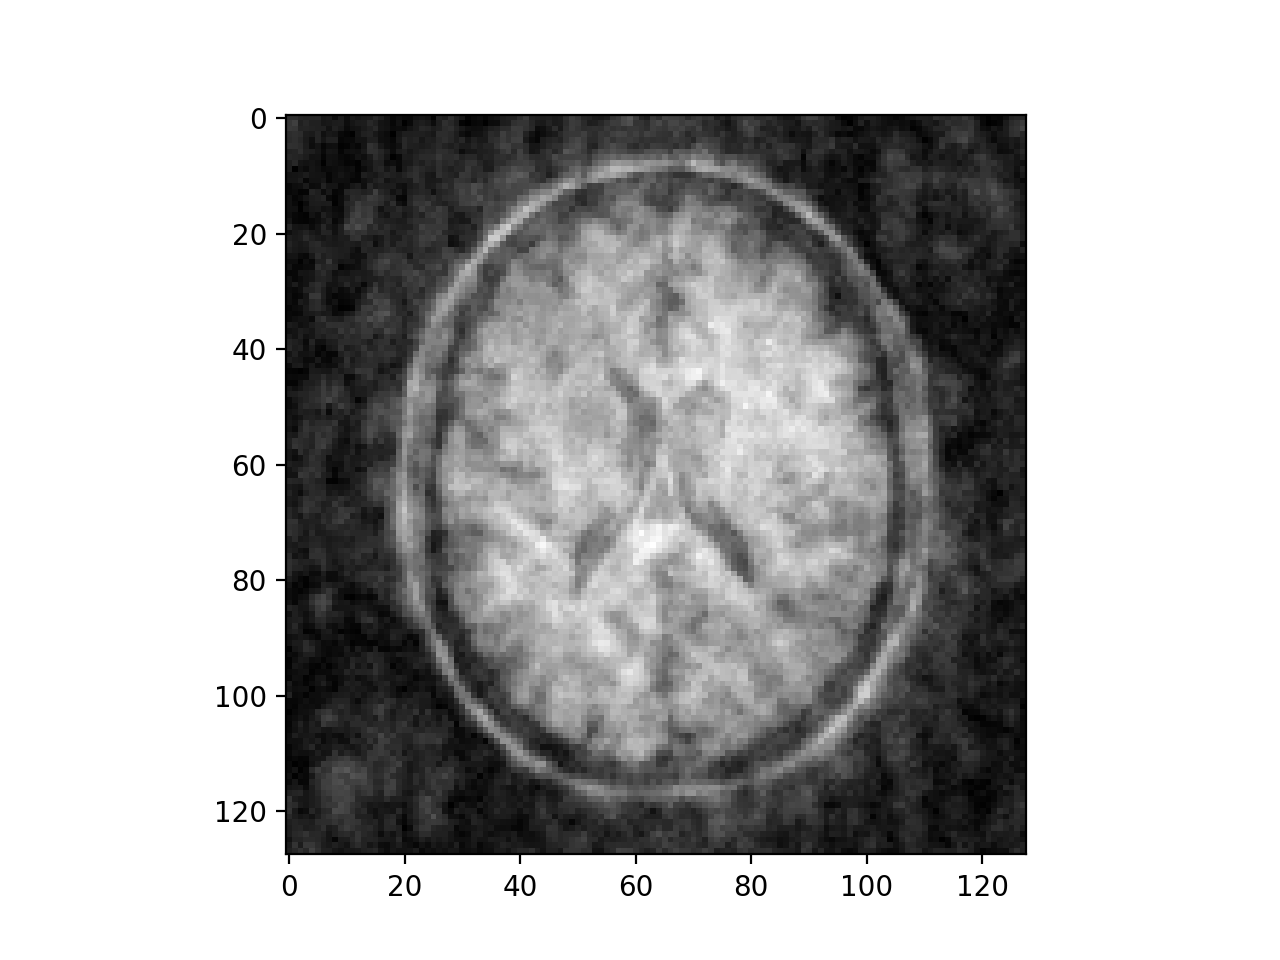
\includegraphics[width=0.5\textwidth]{figs/brain_before.png}
\caption{\label{fig:BrainBefore}Noisy Brain}
\end{figure}

You can consider \ref{fig:BrainBefore} to be the equivalent to a naively
reconstructed image without de-noising. Since we have access to this image, we
can improve our de-noising method by first masking the relevant parts of the
image before converting the data back into k-space via a Fourier Transform,
i.e., see figure \ref{fig:ImageMask}

\begin{figure}[!htpb]
\centering
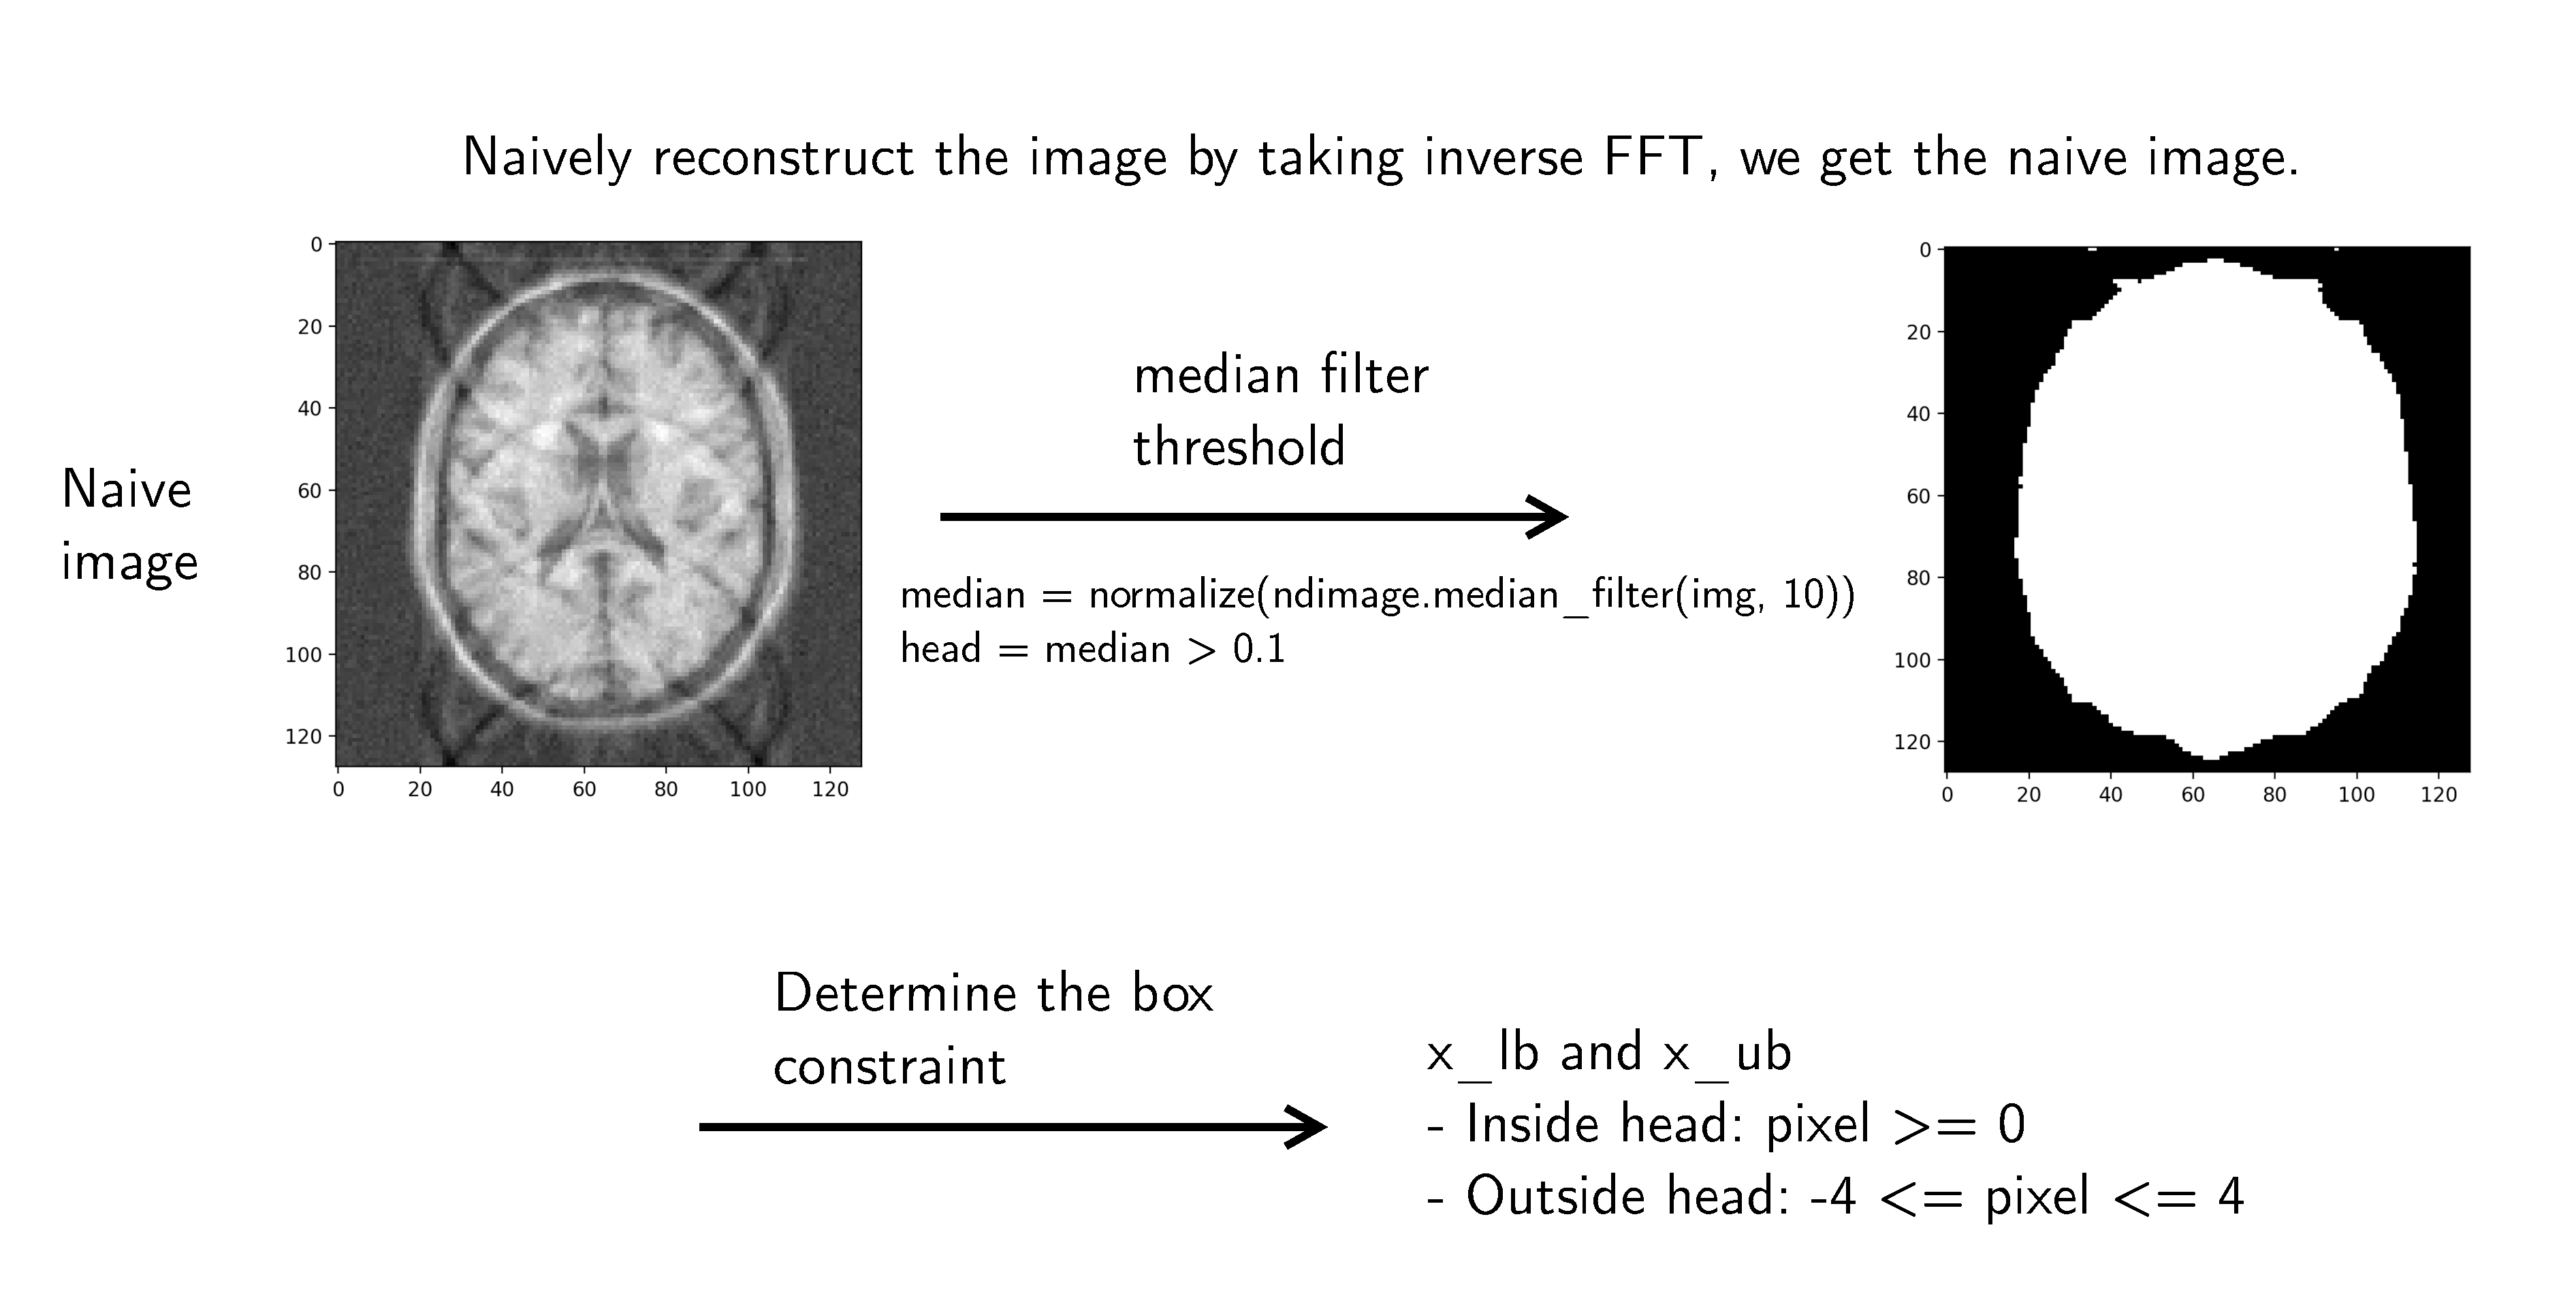
\includegraphics[width=0.8\textwidth]{figs/MRIBrain2.pdf}
\caption{\label{fig:ImageMask}Image Mask}
\end{figure}

We can now solve our image via the following HashedExpression code, which
provides a nice, high level interface for coding our optimization model. Note,
HashedExpression only generates code for computing the objective,constraint
and derivative functions, we then run those code via the IPOPT solver which
uses the interior point algorithm.

\begin{listing}[htbp]
\begin{minted}[]{haskell}
brainReconstructFromMRI :: OptimizationProblem
brainReconstructFromMRI =
  let -- variables
      x = variable2D @128 @128 "x"
      --- bound
      xLowerBound = bound2D @128 @128 "x_lb"
      xUpperBound = bound2D @128 @128 "x_ub"
      -- parameters
      im = param2D @128 @128 "im"
      re = param2D @128 @128 "re"
      mask = param2D @128 @128 "mask"
      -- regularization
      regularization = norm2square (rotate (0, 1) x - x)
                     + norm2square (rotate (1, 0) x - x)
      lambda = 3000
   in OptimizationProblem
        { objective =
            norm2square ((mask +: 0) * (ft (x +: 0) - (re +: im)))
              + lambda * regularization,
          constraints =
            [ x .<= xUpperBound,
              x .>= xLowerBound
            ],
          values =
            [ im :-> VFile (HDF5 "kspace.h5" "im"),
              re :-> VFile (HDF5 "kspace.h5" "re"),
              mask :-> VFile (HDF5 "mask.h5" "mask"),
              xLowerBound :-> VFile (HDF5 "bound.h5" "lb"),
              xUpperBound :-> VFile (HDF5 "bound.h5" "ub")
            ]
        }
\end{minted}
\caption{De-noising HashedExpression Model}
\end{listing}

Running the problem via IPOPT and generating an image from the output yields
the following result, a thoroughly de-noised version of our brain

\begin{figure}[!htpb]
\centering
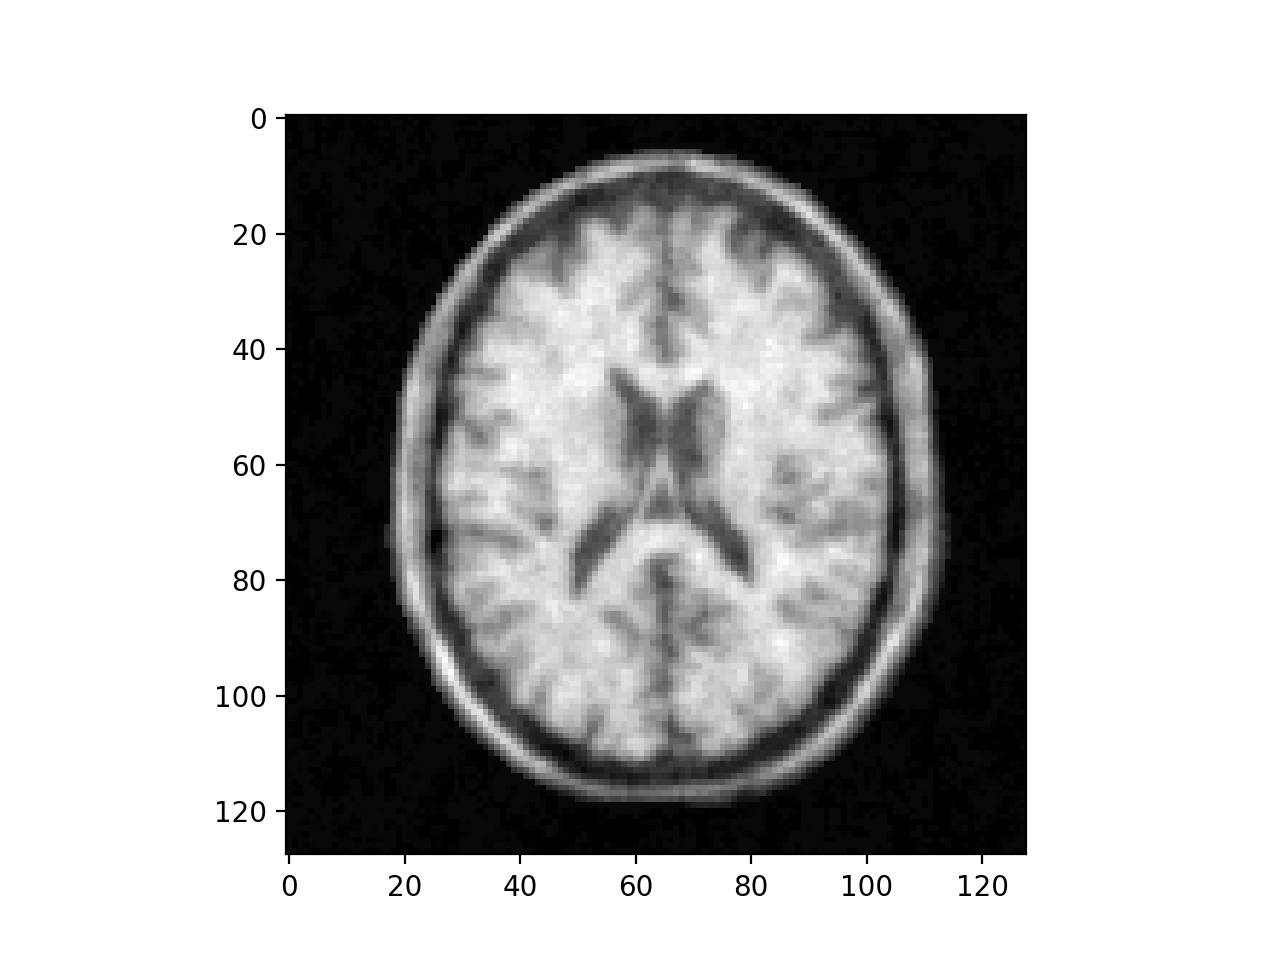
\includegraphics[width=0.5\textwidth]{figs/brain_after.png}
\caption{\label{fig:BrainAfter}De-noised Brain}
\end{figure}

\section{Multi-Coil Sensitivity Reconstruction}
\label{sec:orgf592721}
Real MRI machines use multiple coils to collect data. Each of these coils have
different sensitivities and hence need to be combined while also solving for
the sensitivity of each coil. Say we have two coils A and B, the sensitivity
problem will attempt to solve for the sensitivity of the two coils while
solving for each pixel (say P1/P2) in the resulting image, i.e,

\begin{align}
P1 &= A \cdot S_{1A} + B \cdot S_{1B} \\
P2 &= A \cdot S_{2A} + B \cdot S_{2B} \\
...
\end{align}

To illustrate this problem, I present the following real data collected from
an MRI with 7 different coils. Figure \ref{fig:FruitKSpace} is the summed data in k-space

\begin{figure}[!htpb]
\centering
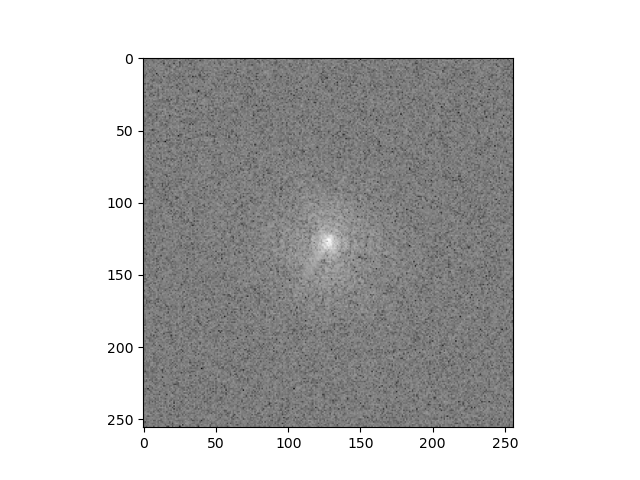
\includegraphics[width=0.5\textwidth]{figs/FruitKSpace.png}
\caption{\label{fig:FruitKSpace}Fruit K Space}
\end{figure}

\newpage
And Figure \ref{fig:NaiveFruit} is the naive reconstruction of the fruit
\begin{figure}[!htpb]
\centering
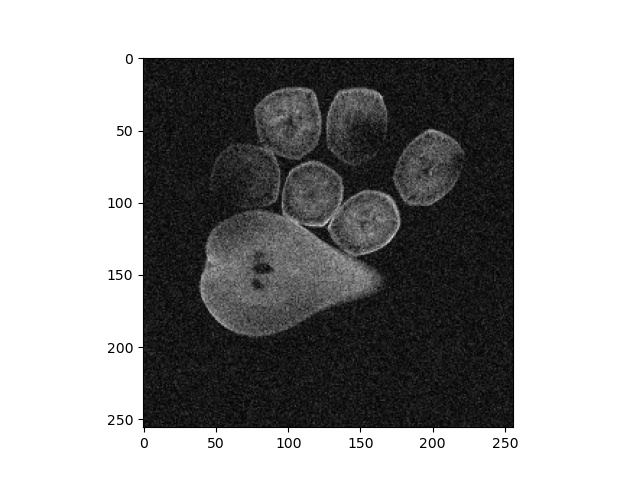
\includegraphics[width=0.5\textwidth]{figs/FruitNaiveReconstruction.png}
\caption{\label{fig:NaiveFruit}Naive Fruit Reconstruction}
\end{figure}


I did not attempt to solve the sensitivity problem directly, but the following
HashedExpression model solves the image using the sum of each of the coils
while regularizing to smooth
\begin{listing}[htbp]
\begin{minted}[]{haskell}
variables:
  a[256][256] = 0
  b[256][256] = 0

constants:
  im0[256][256] = Dataset("fruit.h5", "im0")
  re0[256][256] = Dataset("fruit.h5", "re0")
  ...
let:
  smootherAX = rotate (0, 1) a + rotate (0, -1) a - 2 *. a
  smootherAY = rotate (0, 1) a + rotate (0, -1) a - 2 *. a
  smootherBX = rotate (1, 0) b + rotate (-1, 0) b - 2 *. b
  smootherBY = rotate (1, 0) b + rotate (-1, 0) b - 2 *. b
  regularization = norm2square smootherAX + norm2square smootherAY
                  + norm2square smootherBX + norm2square smootherBY
  coilSum = (re0 +: im0)
              + (re1 +: im1)
              + (re2 +: im2)
              + (re3 +: im3)
              + (re4 +: im4)
              + (re5 +: im5)
              + (re6 +: im6)
              + (re7 +: im7)

minimize:
  norm2square (ft (a +: b) - coilSum)
    + 10000*regularization
\end{minted}
\caption{Multi-Coil HashedExpression Image Reconstruction Model}
\end{listing}

\newpage
Running the optimization using the IPOPT solver generates the following
de-noised image

\begin{figure}[!htpb]
\centering
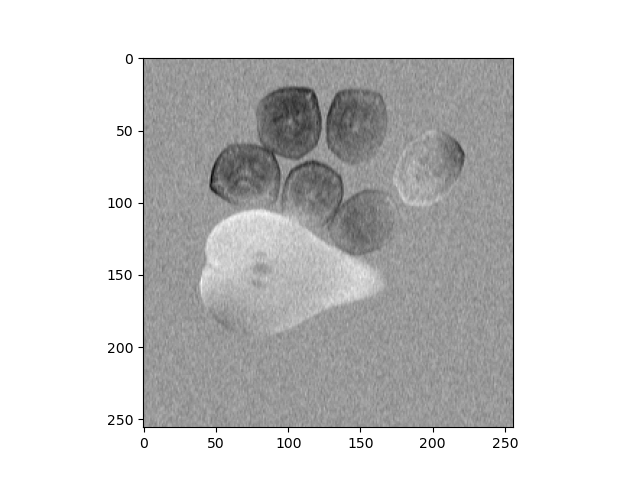
\includegraphics[width=0.5\textwidth]{figs/FruitReconstruction.png}
\caption{\label{fig:FruitReconstruction}Multi-Coil Fruit Reconstruction}
\end{figure}
\end{document}